\documentclass[12pt]{article}

\usepackage{fullpage}
\usepackage{multicol, multirow}
\usepackage{tabularx}
\usepackage{standalone}
\usepackage{listings}
\usepackage{ulem}
\usepackage{amsmath}
\usepackage{pdfpages}
\usepackage[utf8]{inputenc}
\usepackage[russian]{babel}

\newcommand{\StudentName}{Ильвохин Дмитрий}
\newcommand{\Group}{1O-106М}
\newcommand{\CourseName}{Программирование игр}
\newcommand{\LabNum}{5}
\newcommand{\Subject}{Полет в туннеле}
\newcommand{\PrepName}{Аносова Н.\,П.}

\begin{document}

%\documentclass[a4paper, 12pt]{report}
\usepackage[english, russian]{babel}
\usepackage[utf8]{inputenc}
\usepackage{amssymb, amsfonts, amsmath, mathtext, cite, enumerate, float}
\usepackage{geometry}
\usepackage{chngpage}

\begin{document}

\begin{titlepage}

\newpage

\begin{center}
Московский Авиационный Институт \\*
(национальный исследовательский университет) \\*
Факультет прикладной математики и физики \\*
\hrulefill
\end{center}

\begin{center}
Кафедра вычислительной математики и программирования
\end{center}

\vspace{6em}

\begin{center}
\Large \CourseName \\
	Курсоваой проект \\
  <<\Subject>>
\end{center}

\vspace{2em}
\vspace{6em}

\begin{flushright}
	\StudentName, \\
	группа: \Group \\
\vspace{1em}
преподаватель:\\
   \PrepName \\
\end{flushright}

\vspace{\fill}

\begin{center}
Москва, 2015
\end{center}

\end{titlepage}

\end{document}
 % title page

\lstset
{
        language=Python,
        basicstyle=\footnotesize,% basic font setting
        extendedchars=\true
}

\begin{flushright}
\Large{
	\CourseName \\
	Лабораторная работа №\,\LabNum \\
	<<\Subject>> \\
  \StudentName, \Group \\
}
\end{flushright}

\subsection*{Задание}
Требуется реализовать игру: шарик, за которым находится камера, движется
по бесконечному туннелю. В туннеле возникают препятствия, которые необходимо
обходить управляя шариком. Количество столкновений шарика с препятствием
нужно подсчитывать.

\subsection*{Практическая часть}
Для выполнения лабораторной работы решил опять использовать
игровой движок Padna3D.

За основу был взят обучающий пример из обучающий примеров Panda3D.

Основная идея следующая: генерируется три части туннеля, которые ставятся друг
за другом. Каждый туннель с определенной скоростью движется вдоль оси $Z$.
Как только часть туннеля перестает быть видимой --- она перемещается за двумя другими
частями туннеля вперед. Действие повторяется бесконечно, создавая видимость бесконечного
движения в туннеле.

Для того, чтобы скрыть момент перемещения новой части туннеля --- добавлен эффект тумана.

Препятствиями служат модели кристаллов, взятые из коллекции моделей Panda3D.
Они генерируются случайным образом в момент перемещения текущей части туннеля в конец.

Счетчик столкновений выводится в консоль.

\begin{figure}[!htb]
  \centering
    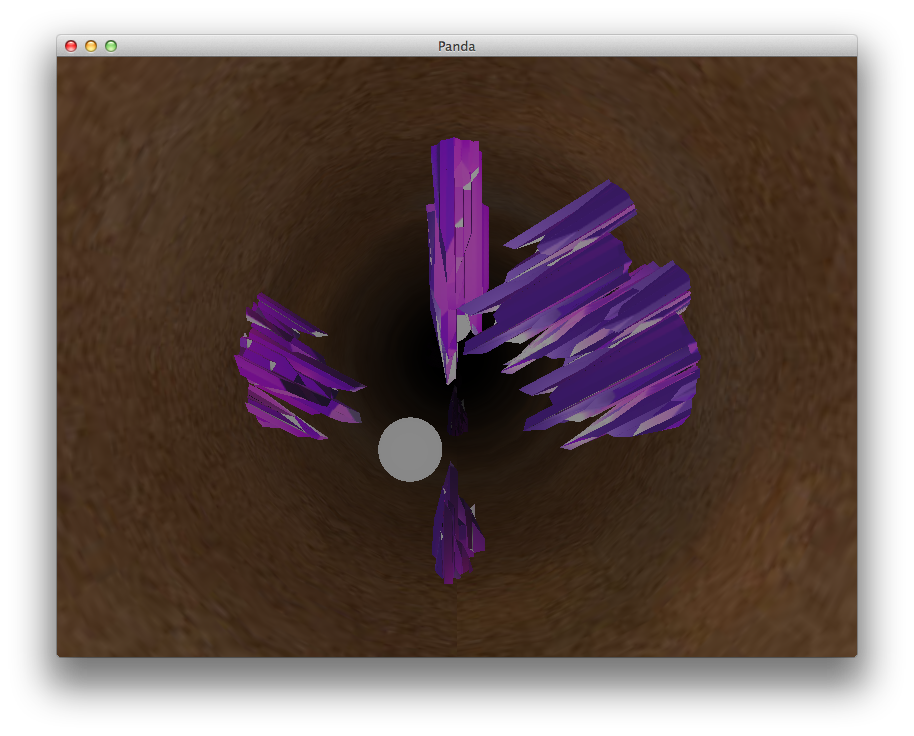
\includegraphics[scale=0.5]{pics/game.png}
   \caption{Скриншот}
    \label{fig:game}
\end{figure}

% Сомнительный вывод, но какой есть (%
\subsection*{Выводы}
Модель кристалла, которая используется в качестве препятствия состоит примерно
из 17 тысяч полигонов и проверять коллизии относительно каждого полигона довольно
дорого. На моем ноутбуке начинались ощутимые тормоза уже при пяти препятствиях.
Поэтому решил использовать Bounding Box'ы и проверять коллизии относительно них.
Получилось намного быстрее, но из-за этого пострадала точность коллизий, иногда,
пролетая мимо кристалла можно случайно зацепить его Bounding Box и столкновение
засчитается.

\begin{thebibliography}{}
\bibitem{panda_wiki} https://ru.wikipedia.org/wiki/Panda3D
\bibitem{panda} https://www.panda3d.org/
\end{thebibliography}

\end{document}

